\documentclass{standalone}
\usepackage{tikz}
\usepackage{amsmath}
\usepackage{xcolor}
\usetikzlibrary{arrows.meta, decorations.pathreplacing, backgrounds, positioning, calc}
% Define custom colors
\definecolor{softyellow}{HTML}{F2D648}
\definecolor{dustyblue}{HTML}{9EB9D4}
\definecolor{berkeleyblue}{RGB}{0, 50, 98}
\definecolor{berkeleygold}{RGB}{253, 181, 21}

\begin{document}

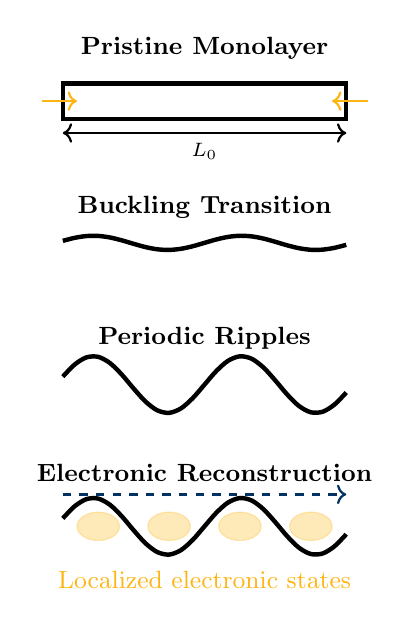
\begin{tikzpicture}[scale=0.9]

  % Pristine monolayer
  \node at (0,3) {\small \textbf{Pristine Monolayer}};
  \draw[ultra thick] (-2,2.5) rectangle (2,2);
  \draw[<->, thick] (-2,1.8) -- (2,1.8) node[midway, below] {\scriptsize $L_0$};
  \draw[->, thick, berkeleygold] (-2.3,2.25) -- (-1.8,2.25);
  \draw[->, thick, berkeleygold] (2.3,2.25) -- (1.8,2.25);

  % Buckling
  \node at (0,0.75) {\textbf{\small Buckling Transition}};
  \draw[ultra thick] plot[smooth, domain=-2:2] (\x, {0.25+0.1*sin(3*\x r)});

  % Periodic ripples
  \node at (0,-1.1) {\textbf{\small Periodic Ripples}};
  \draw[ultra thick] plot[smooth, domain=-2:2] (\x, {-1.75+0.4*sin(3*\x r)});

  % Electronic Reconstruction
  \node at (0,-3) {\textbf{\small Electronic Reconstruction}};
  \draw[ultra thick] plot[smooth, domain=-2:2] (\x, {-3.75+0.4*sin(3*\x r)});

  % Localized states
  \foreach \x in {-1.5,-0.5,0.5,1.5} {
    \filldraw[berkeleygold, opacity=0.3] (\x,-3.75) ellipse (0.3 and 0.2);
  }
  \node[anchor=north] at (0,-4.25) {\scriptsize \textcolor{berkeleygold}{\small Localized electronic states}};

  % Electron transport arrow
  \draw[->, thick, dashed, berkeleyblue] (-2,-3.3) -- (2,-3.3);

\end{tikzpicture}

\end{document}
